\documentclass[8pt,handout]{beamer}
%\usetheme{Pittsburgh}
\usetheme{Singapore}
\usepackage{CJKutf8}

\begin{document}
\begin{CJK*}{UTF8}{gkai}
\begin{frame}{}
\begin{columns}
	\column{7cm}
	\begin{itemize}
		\item {\bf\large xiayf},25岁,xxx
		\item 目前就读于{\large\color{blue}xxxx}软件学院,{\large\color{blue}{研二}}
		\item 联系方式: 159xxx84916, xxxxxx@xxxx.edu.cn 
	\end{itemize}
	\column{3cm}
		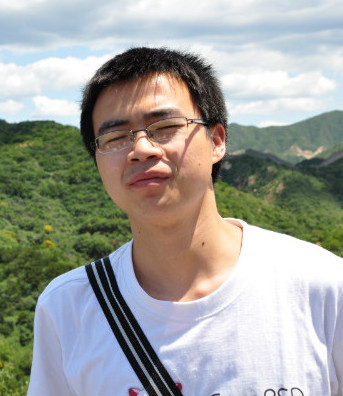
\includegraphics[width=1.8cm]{xiayf.jpg}
\end{columns}
\begin{block}{技术能力}
\begin{itemize}
	\item 熟悉Python, C, Java,了解PHP,shell,scheme,go
	\item 熟悉Unix/linux系统管理,系统编程\\(一年半Ubuntu,一年Debian,ArchLinux使用经验,FreeBSD新手)
	\item 熟练运用常用数据结构与算法
	\item 具备一定的web开发经验
	\item 英语水平6级,英文阅读能力较好
\end{itemize}
\end{block}
\begin{block}{项目经验}
\begin{itemize}
	\item 2012.2至今 : {\color{blue}{基于Web的群体机器人远程控制系统}}
	\item 2011.6 - 2011.10 : {\color{blue}{机器人多目标跟踪}}
	\item 2010.11 - 2011.4 : {\color{blue}{群体机器人程序批量烧录}}
	\item 实验室ftp服务辅助工具---简易ftp搜索引擎
	\item 本科毕业论文---基于heritrix的聚焦爬虫开发
\end{itemize}
\end{block}
\end{frame}
\begin{frame}{}
\begin{block}{专业核心课程}
\begin{itemize}
	\item 高级操作系统,算法设计与分析,海量信息处理,计算机体系结构,软件工程
\end{itemize}
\end{block}
\begin{block}{个人获奖情况}
\begin{itemize}
	\item 2010-2011: 香港道德基金会奖学金
	\item 2011-2012: 香港道德基金会奖学金
	\item 2008-2009: 上海大学自强不息奖学金,国家励志奖学金
	\item 2007-2008: 上海大学国家励志奖学金,军训优秀导生标兵
	\item 2006-2007: 上海大学二等奖学金,国家励志奖学金,校优秀学生
\end{itemize}
\end{block}
\begin{block}{社会实践}
\begin{itemize}
	\item 2011.3至今:实验室服务器管理员
	\item 2011.9 - 2012.1: 交大-致远学院-计算机科学导论课程-助教
	\item 2011.3 - 2011.7: 交大-本科ACM班-计算机组成课程-助教
	\item 2011.3 - 2011.7: 交大-软件学院教务办-助管
	\item 2007 - 2008: 上海大学-计算机学院-学生会宣传部-部长
\end{itemize}
\end{block}
\end{frame}
\end{CJK*}
\end{document}
